\chapter{Implementation}
\label{chap:experimental_setup}

% =====================================================================
% CHAPTER SCAFFOLD (structure agreed in outline).
% Headings (\section/\subsection/\paragraph) are REAL; per-part guidance
% is in % comments. Existing drafted prose, tables and figures are kept.
% Tags: [NEW] gap | [MOVE] relocate | [SHIFT] project pivot | [EXISTS] keep.
% Splitting rule -- this chapter = HOW EXACTLY (engineering level,
% reproducible). Conceptual framing / WHY lives in Methodology (Chapter 3).
% Section order: 4.1 plant LSTMs | 4.2 efficiency | 4.3 Gym env |
% 4.4 algorithms | 4.5 HPO | 4.6 infrastructure | 4.7 per-phase pipelines.
% =====================================================================

This chapter describes the implementation of the experimental framework used to train and evaluate the reinforcement-learning controllers. It first introduces the \ac{LSTM}-based vehicle-model stack, including its interfaces, validity ranges, recurrent-state initialisation, and deployment optimisations that make large-scale \ac{RL} training computationally feasible. The chapter then details the custom Gymnasium \cite{towers_gymnasium_2024} environment that connects the surrogate models to the learning agents by defining the observation space, action mapping, reward function, safety mechanisms, and episode structure.

The remaining sections describe the concrete \ac{RL} algorithm implementations, the hyperparameter-optimisation procedure, the training infrastructure, and the two-stage experimental pipeline. In this way, the chapter provides the engineering-level details required to reproduce the Phase~1 speed-tracking experiments and the Phase~2 emission- and \ac{SOC}-aware fine-tuning experiments.

% The LSTM-based plant surrogates used in this work were trained on transient data generated from separated GT-Suite submodels for the ICE and the PG/drivetrain system \cite{frey_data-based_2025}. To improve coverage of the operating space, the data-generation workflow used automatically generated random time series composed of smooth ramps and random jumps, with ambient conditions kept constant over each cycle and the initial SoC treated as a cycle-level condition. In the setup reported by Frey et al., this produced 93 ICE cycles and 3,630 PG-EM cycles of 1,800 seconds each. The resulting time series were resampled to 2~Hz, cleaned for outliers, scaled to the interval $[-1,1]$ with a Min-Max scaler, and then split into training, validation, and test subsets. The ICE data used a 70/20/10 split, whereas the PG-EM data used a 50/30/20 split. For training, LSTM networks with AdamW optimisation, batch size 1, and MAE loss were used, while hidden-state initialisation was improved using the auxiliary-state method proposed by Hagenbucher et al. \cite{hagenbucher_initialization_2023}. \autoref{tab:lstm_training_hyperparameters} summarises the architectures and hyperparameters reported for the trained subnetworks.

% An important architectural finding from the cascaded-network study is that the physically intuitive first cascade design led to unstable carrier-speed prediction and oscillatory closed-loop behaviour. For this reason, the revised Model~2 formulation was preferred: instead of predicting the carrier-speed feedback internally, it uses the $n_{ICE}$ target directly as a shared input to both subnetworks. This removes the problematic internal feedback loop, improves robustness, and is therefore the relevant basis for the RL-oriented plant-model deployment described in the following subsection \cite{frey_data-based_2025}.

% ---------------------------------------------------------------------
\section{The Specific Vehicle LSTMs}
\label{sec:impl_lstms}
% [EXISTS, strong] Provenance, architectures, validity ranges, I/O, init.
The vehicle-model stack used in this work consists of recurrent \ac{LSTM} surrogate models provided by Frey et al. \cite{frey_data-based_2025}. These models represent the EA189 \ac{ICE} with a customised aftertreatment setup and the drivetrain. The \ac{LSTM} network training configurations are described in \autoref{tab:lstm_model_architectures}.

\begin{table}[H]
  \centering
  \begin{tabular}{|l|l|l|l|}
    \hline
    \textbf{Parameter} & \textbf{ICE} & \textbf{Drivetrain} & \textbf{Drivetrain Plus} \\
    \hline
    Layers & 3 & 3 & 3 \\
    Neurons per layer & 256 & 256 & 256 \\
    Sequence length [s] & 600 & 1800 & 1800 \\
    Batch size & 1 & 1 & 1 \\
    Optimiser & AdamW & AdamW & AdamW \\
    Initial learning rate & 1e-3 & 1e-3 & 1e-3 \\
    Scaler & Min-max-scaler & Min-max-scaler & Min-max-scaler \\
    Loss function & MAE & MAE & MAE \\
    \hline
  \end{tabular}
  \caption[Surrogate LSTM architectures and hyperparameters]{Neural network architectures and training hyperparameters of the LSTM surrogate models used in this work.}
  \label{tab:lstm_model_architectures}
\end{table}

The underlying numerical plant models were implemented in GT-Suite \cite{gamma_technologies_gt-suite_nodate} to generate synthetic data for training the LSTM surrogates. These are characterised by the following properties:

\paragraph{Cascaded architecture.}
The final model stack consists of three neural networks: an \emph{ICE} network, a \emph{Drivetrain} network, and the optional \emph{Drivetrain Plus} network, as illustrated in \autoref{fig:nn_model_architecture_placeholder}. The ICE network receives engine speed ($n_{ICE}$), fuel mass ($m_{fuel}$), ambient temperature ($T_{amb}$), and ambient pressure ($p_{amb}$) as inputs and predicts engine torque ($\tau_{ICE}$) as the transfer output, together with emissions- and aftertreatment-related variables.

The drivetrain network receives $n_{ICE}$, $\tau_{ICE}$, EM2 torque ($\tau_{EM2}$), and mechanical braking (\texttt{Brakemech}) as inputs and predicts vehicle speed ($v_{Car}$) and battery state of charge ($SoC$). For RL purposes, $v_{Car}$ and $SoC$ are the key plant outputs required to evaluate tracking performance, energy usage, and the feasibility of the control action. Ambient conditions are assumed to remain constant over one complete driving cycle of 1800 seconds, with valid ranges of 250--310 K for $T_{amb}$ and 0.8--1.1 bar for $p_{amb}$.

An exhaustive overview of the network interfaces of the \ac{ICE}, Drivetrain, and Drivetrain Plus neural networks is provided in Appendix~\ref{app:model_interfaces}; \autoref{tab:ice_io}, \autoref{tab:drivetrain_io}, and \autoref{tab:drivetrain_plus_io}.

\begin{figure}[htbp]
  \centering
  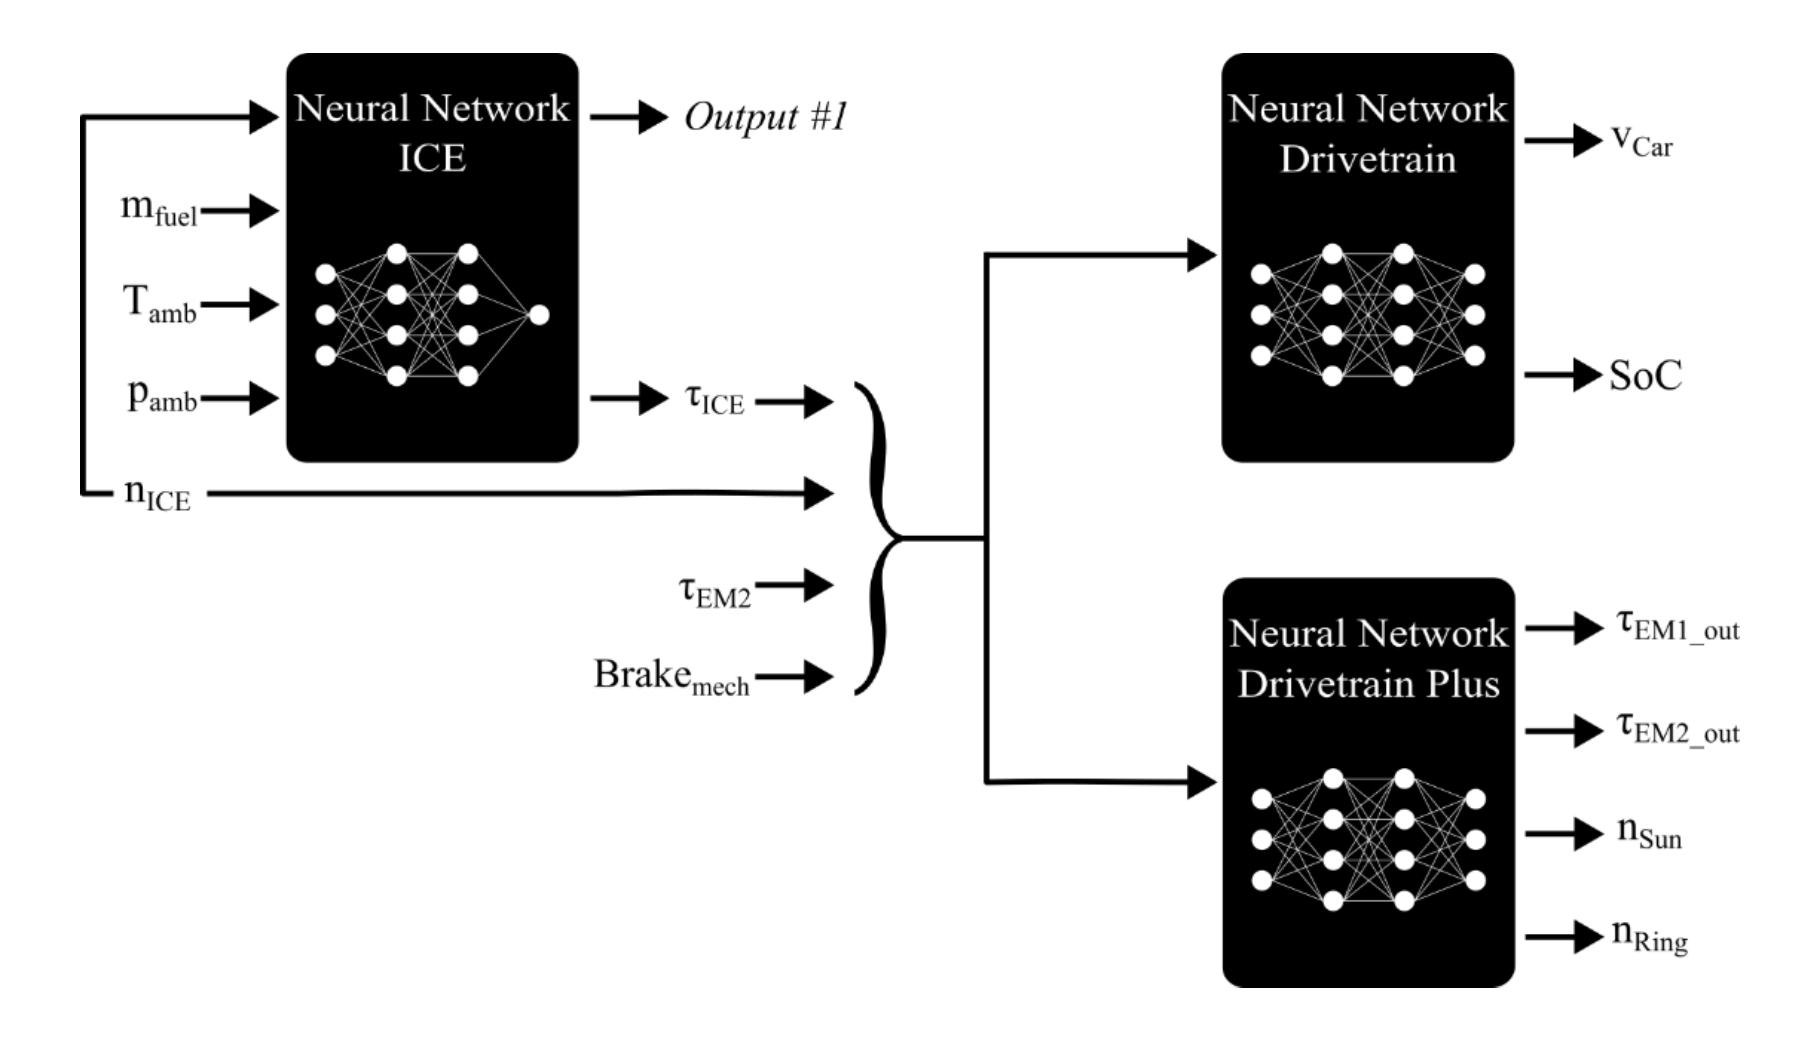
\includegraphics[width=0.65\textwidth]{imgs/lstm_flow.png}
  \caption[Cascaded surrogate LSTM architecture]{Final version of the cascaded surrogate LSTM architecture; reprinted from \cite{frey_data-based_2025}.}
  \label{fig:nn_model_architecture_placeholder}
\end{figure}

\paragraph{Validity ranges.}
The latest models represent cooldown behaviour during engine-off phases by including stationary cooldown cycles in the training set. Consequently, the ICE model has two distinct valid operating regimes: engine-off operation with $n_{ICE}=0$ rpm and $m_{fuel}=0$, and engine-on operation in the range $900\,\text{rpm} \leq n_{ICE} \leq 4000\,\text{rpm}$ with $3\,\text{mg} \leq m_{fuel} \leq 70\,\text{mg}$. The intermediate region between engine-off and engine-on conditions is explicitly invalid, meaning operation between 0 and 900 rpm or between 0 and 3 mg fuel mass is not supported and may produce unphysical behaviour. The operating ranges of the \ac{ICE} and drivetrain models are summarised in \autoref{tab:ice_valid_ranges} and \autoref{tab:dt_valid_ranges}.

\begin{table}[H]
  \centering
  \begin{tabular}{|l|l|}
    \hline
    \textbf{Parameter} & \textbf{Range} \\
    \hline
    Speed ($n_{ICE}$) & Engine off: 0 rpm; engine on: 900--4000 rpm \\
    Fuel mass ($m_{fuel}$) & Engine off: 0 mg; engine on: 3--70 mg \\
    Ambient temperature ($T_{amb}$) & 250--310 K \\
    Ambient pressure ($p_{amb}$) & 0.8--1.1 bar \\
    \hline
  \end{tabular}
  \caption[ICE model valid ranges]{Valid ranges of the ICE model.}
  \label{tab:ice_valid_ranges}
\end{table}

\begin{table}[H]
  \centering
  \begin{tabular}{|l|l|}
    \hline
    \textbf{Parameter} & \textbf{Range} \\
    \hline
    State of charge ($SoC$) & 0--1 \\
    Engine speed ($n_{ICE}$) & 0--4500 rpm \\
    EM2 torque ($\tau_{EM2}$) & $-421$ to 421 Nm \\
    ICE torque ($\tau_{ICE}$) & $-50$ to 300 Nm \\
    Mechanical brake (\texttt{Brakemech}) & 0--100\% \\
    \hline
  \end{tabular}
  \caption[Drivetrain model valid ranges]{Valid ranges of the drivetrain model.}
  \label{tab:dt_valid_ranges}
\end{table}

\paragraph{Initialisation of the LSTMs.}
All recurrent models use a \emph{two-part} LSTM scheme, with a dedicated initialisation model and an inference model, to prevent recurrent inference from starting with arbitrary hidden states. By default, these states are initialised to zero, which can result in a warm-up phase with reduced prediction accuracy. Frey et al. \cite{frey_data-based_2025} followed Hagenbucher et al. \cite{hagenbucher_initialization_2023} to address this issue by the \emph{two-parted} intitialisation. The initial timestep is handled by a separate initialisation model that maps physically meaningful initial conditions to the internal LSTM state required by the inference model.

\paragraph{Drivetrain Plus network.} The vehicle-model stack includes an additional \emph{Drivetrain Plus} network, whose interface is summarised in Appendix~\ref{app:model_interfaces}; \autoref{tab:drivetrain_plus_io}. It uses the same inputs as the standard drivetrain model but predicts additional internal drivetrain variables. It is not required for the present RL control loop, but it allows for richer state diagnostics and more interpretable post-analysis of drivetrain operation.

% ---------------------------------------------------------------------
\section{Computational Efficiency and Deployment}
\label{sec:impl_efficiency}
The vehicle-model stack provides a computationally efficient surrogate environment for \ac{RL} experiments, but achieving this throughput required particular deployment optimisations. Since \ac{RL} training depends directly on the rate of plant-model inference, these inference-performance gains are indispensable for the present work.

\paragraph{Model execution mode.} Inference time was a major bottleneck in previous project iterations (\autoref{subsec:current_limitations}). The main improvement was achieved by utilising the \texttt{tf.function} decorator, which enables TensorFlow to compile the Python code into a highly optimised computation graph. Instead of relying on Python's default eager execution to evaluate operations step by step, this approach traces the function once and reuses the pre-compiled graph for subsequent calls. This bypasses the Python interpreter overhead and allows for graph-level optimisations, significantly accelerating inference times \cite{geeksforgeeks_tffunction_nodate}. On the \ac{WLTC}, this reduced the total rollout time from 104.50~s to 4.79~s in a local MacBook benchmark (\autoref{fig:tf_runtime_benchmarks}).

\begin{figure}[H]
  \centering
  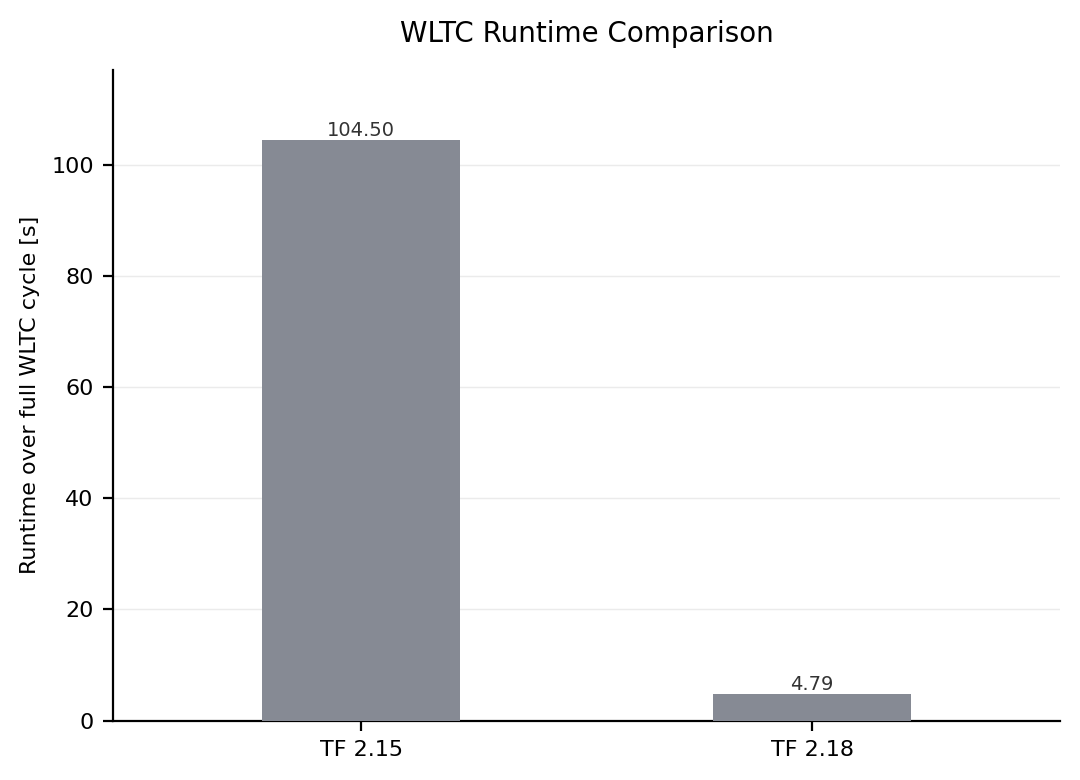
\includegraphics[width=0.6\textwidth]{imgs/WLTC_runtime_clean.png}
  \caption[WLTC speed up benchmark]{Total runtime over the full WLTC cycle executed on a 2023 Macbook Pro with a speed up of more than $20\times$.}
  \label{fig:tf_runtime_benchmarks}
\end{figure}

\paragraph{Model file switch.} Following the recommendations of researchers at CTTC-UPC \cite{centre_tecnologic_de_transferencia_de_calor_cttc-upc_heat_2026}, the models were converted from TensorFlow to a language- and framework-agnostic format to improve portability across execution environments. Since no automatic conversion was available for the models used here, CTTC-UPC implemented ad hoc export routines and developed a high-level library that emulates the TensorFlow interface, enabling seamless model replacement. This produced additional performance gains which, although smaller than the graph-mode improvement described above, still contribute meaningfully to efficient \ac{RL} training (\autoref{fig:scaler_model_speedups}).

\begin{figure}[H]
  \centering
  \begin{subfigure}[t]{0.44\textwidth}
    \centering
    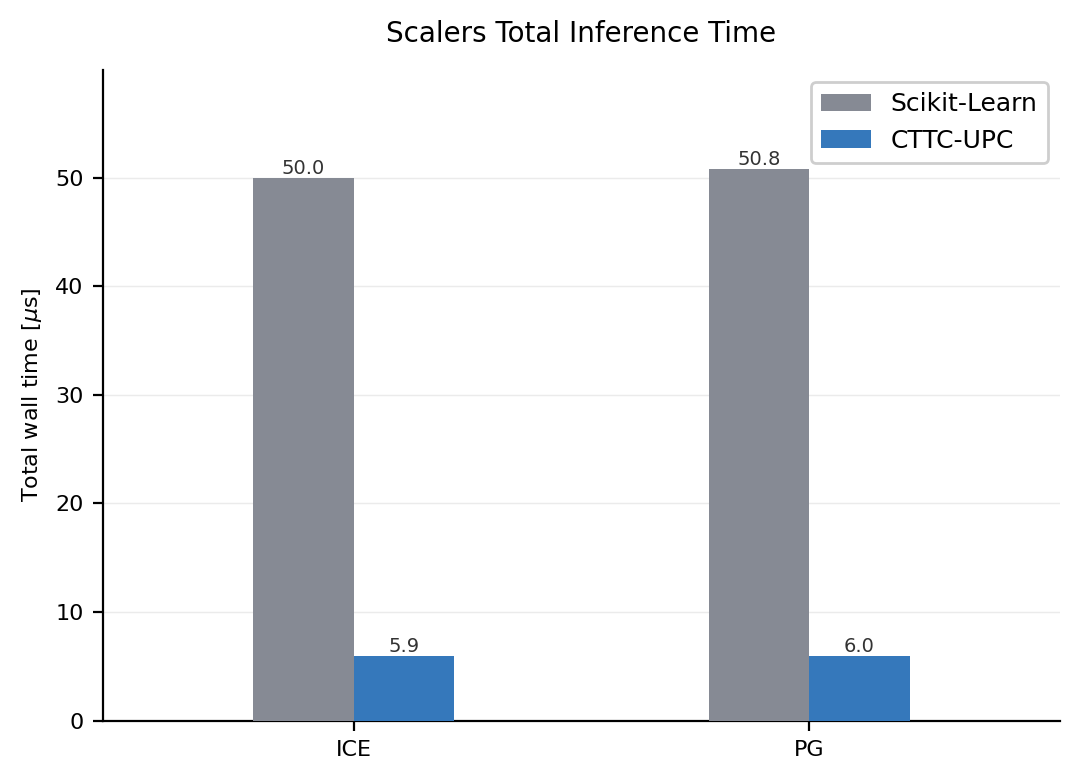
\includegraphics[width=\textwidth]{imgs/scalers_speedup_clean.png}
    \caption[Scaler overhead speed up]{Total scaler overhead per control step, obtained by summing the three scaler operations per inference call: forward input transformation, inverse output transformation, and forward output transformation. The speed up corresponds to approximately $8.5\times$.}
  \end{subfigure}
  \hfill
  \begin{subfigure}[t]{0.54\textwidth}
    \centering
    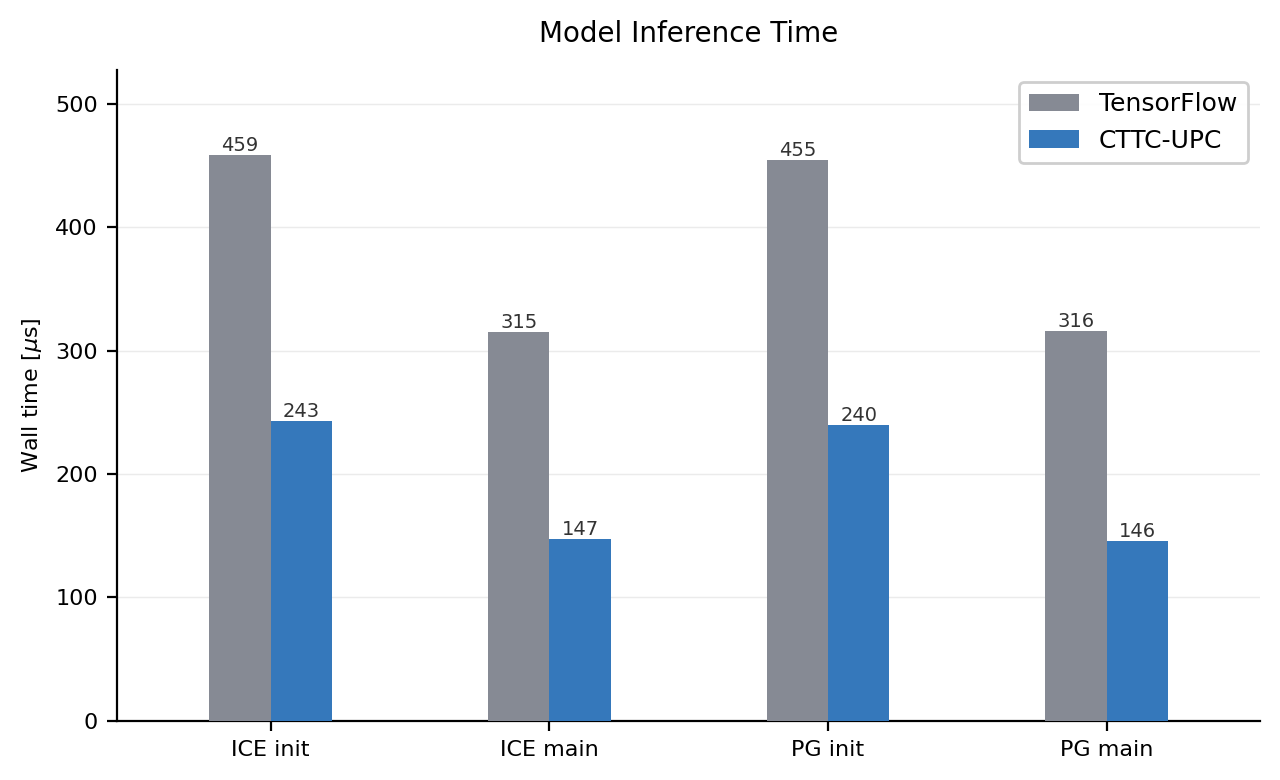
\includegraphics[width=\textwidth]{imgs/models_speedup_clean.png}
    \caption[Model execution speed up]{Forward-pass latency for the initialisation and inference model, yielding approximately $2\times$ speed ups, respectively.}
  \end{subfigure}
  \caption[Inference-speedup comparison]{Wall-clock inference time of the original Scikit-Learn/TensorFlow implementations versus the optimised CTTC-UPC \cite{centre_tecnologic_de_transferencia_de_calor_cttc-upc_heat_2026} counterparts.}
  \label{fig:scaler_model_speedups}
\end{figure}

% ---------------------------------------------------------------------
\section{The Reinforcement-Learning Environment}
\label{sec:impl_environment}
After the surrogate \ac{LSTM}s have been validated, they cannot simply be connected directly to the \ac{RL} agent. Instead, a custom Gymnasium \cite{towers_gymnasium_2024} environment is required to wrap the cascaded \ac{LSTM} stack and define the essential elements of \ac{RL}: observations, actions, and rewards.

\paragraph{Observation space.}
The agent observes a $12$-dimensional vector that instantiates the four conceptual groups defined in \autoref{subsec:method_observation}. Its components, their physical units and the per-component bounds used for the subsequent normalisation are listed in \autoref{tab:obs_vector}. The bounds are chosen to comfortably enclose the operating range (based on the requirements defined by \cite{frey_data-based_2025}), supported by the surrogate networks (\autoref{sec:impl_lstms}) and the limit values exposed by the action interface.

\begin{table}[H]
  \centering
  \small
  \begin{tabular}{|c|l|l|l|c|c|}
    \hline
    \textbf{\#} & \textbf{Symbol} & \textbf{Description} & \textbf{Unit} & \textbf{Low} & \textbf{High} \\
    \hline
    1  & $v_{Car}$              & Vehicle speed                          & km/h     & $-5$    & $150$   \\
    2  & $\Delta v$              & Speed error w.r.t.\ target             & km/h     & $-155$  & $155$   \\
    3  & $\mathrm{SOC}$         & Battery state of charge                & --       & $0$     & $1$     \\
    4  & $\tau_{ICE}$            & ICE torque                             & Nm       & $-50$   & $300$   \\
    5  & $\dot m_{\mathrm{NO}_{x},\mathrm{tp}}$ & Tailpipe NOx mass-flow rate            & g/s      & $0$     & $0.4$   \\
    6  & $n_{ICE}$               & ICE speed                              & rpm      & $0$     & $4000$  \\
    7  & $m_{fuel}$              & Injected fuel mass                     & mg       & $0$     & $70$    \\
    8  & $\Delta\mathrm{SOC}$   & SOC deviation from episode-initial     & --       & $-1$    & $1$     \\
    9  & $\bar t_{\text{eng}}$  & Normalised engine-switch timer         & --       & $0$     & $1$     \\
    10 & $\tau_{EM2}^{-}$        & Last EM2 torque                        & Nm       & $-421$  & $421$   \\
    11 & $u_{\text{brk}}^{-}$    & Last mechanical brake percentage       & \%       & $0$     & $100$   \\
    12 & $T_{\text{wall,SCR1}}$ & SCR1 wall temperature                  & K        & $298$   & $1240$  \\
    \hline
  \end{tabular}
  \caption[Observation-vector components and bounds]{Components of the observation vector, with their physical bounds used for min-max normalisation. The thermal proxy $T_{\text{wall,SCR1}}$ is the single compromise that turns the underlying POMDP into the tractable MDP approximation of \autoref{subsec:method_mdp}.}
  \label{tab:obs_vector}
\end{table}

After clipping each component to $[\text{low},\,\text{high}]$, the observation is min-max-normalised to $[0,\,1]$ and supplied to the policy network as a $\mathbb{R}^{12}$ vector. The engine-switch timer is itself a normalised quantity in $[0,\,1]$ that counts the elapsed steps since the last engine on/off transition and equals $1$ once the engine switch cooldown described below has elapsed.

\paragraph{Action space.}
The agent acts through a four-dimensional continuous Box action in $[-1,\,1]^{4}$. Each component is rescaled per step to its physical range before being passed to the plant, as listed in \autoref{tab:action_space}.

\begin{table}[H]
  \centering
  \small
  \begin{tabular}{|c|l|l|c|c|}
    \hline
    \textbf{\#} & \textbf{Symbol} & \textbf{Description} & \textbf{Agent range} & \textbf{Physical range} \\
    \hline
    1 & $a_{ICE}$          & ICE command (on/off + rpm) & $[-1,\,1]$ & $\{\text{off}\} \cup [900,\,4000]$ rpm \\
    2 & $\tau_{EM2}$        & EM2 torque                 & $[-1,\,1]$ & $[-421,\,421]$ Nm \\
    3 & $m_{fuel}$          & Fuel mass per cycle        & $[-1,\,1]$ & $[3,\,70]$ mg \\
    4 & $u_{\text{brk}}$    & Mechanical brake           & $[-1,\,1]$ & $[0,\,100]\,\%$ \\
    \hline
  \end{tabular}
  \caption[Action-vector components and ranges]{Components of the action vector, with the agent-side normalised range and the physical range after rescaling.}
  \label{tab:action_space}
\end{table}

The ICE command implements the design choice introduced in \autoref{subsec:method_action}: it encodes both the engine on/off decision and the rpm setpoint through the piecewise map
\begin{equation}
  (n_{ICE},\,m_{fuel}) =
  \begin{cases}
    (0,\,0), & a_{ICE} \le 0, \\
    \bigl(900 + a_{ICE}\,(4000 - 900),\;m_{fuel,\text{scaled}}\bigr), & a_{ICE} > 0,
  \end{cases}
  \label{eq:ice_command}
\end{equation}
where $m_{fuel,\text{scaled}}$ is the fuel command after the agent-to-physical rescaling of \autoref{tab:action_space}. The negative half of the ICE command therefore corresponds to engine-off with fuel mass forced to zero, while the positive half spans the LSTM-valid engine speed range $[900,\,4000]\,\text{rpm}$. The intermediate invalid regions of the ICE surrogate (0--900~rpm and 0--3~mg) are unreachable by design.

\paragraph{Reward function.}

The reward emitted each step comprises four conceptual contributions: a Gaussian speed-tracking reward, an emission penalty, a charge-sustaining \ac{SOC} penalty, and a mechanical shaping penalty that regularises engine flickering and braking (which proved necessary in order to stabilise early training),

\begin{equation}
  R_t = \underbrace{W_{\text{speed}} \cdot \exp\!\left(-\frac{1}{2}\left(\frac{\Delta v_t}{\sigma_v}\right)^{2}\right)}_{\text{Speed Tracking}}
  - \underbrace{\left(W_{\text{emi}} \cdot \tilde e_{\mathrm{NO}_{x},t}\right)}_{\text{Emissions}}
  - \underbrace{\left(W_{\text{soc}^2} \cdot (\Delta\text{SOC}_t)^{2}\right)}_{\text{SOC Management}}
  - P_{\text{mech},t},
  \label{eq:reward}
\end{equation}

where $\Delta v_t = v_{\text{ref},t} - v_t$ is the instantaneous speed error, $\Delta\text{SOC}_t = \text{SOC}_t - \text{SOC}_0$ the deviation from the episode-initial \ac{SOC}, and $\tilde e_{\mathrm{NO}_{x},t} = \min\!\bigl(\dot m_{\mathrm{NO}_{x},\mathrm{tp},t} / c_{\mathrm{NO}_{x},\mathrm{rate}},\,1\bigr)$ the clipped normalised tailpipe \ac{NOx} mass-flow rate. The mechanical shaping penalty is

\begin{equation}
  P_{\text{mech},t} = W_{\text{brake}} \cdot \frac{u_{\text{brk},t}}{c_{\text{brk}}}
  + W_{\text{flick}} \cdot \!\left[\text{engine}_t{=}\text{ on}\wedge\text{engine}_{t-1}{=}\text{ off}\right],
  \label{eq:pmech}
\end{equation}

and the fixed normalisation constants take the values $c_{\mathrm{NO}_{x},\mathrm{rate}} = 0.4$~g/s and $c_{\text{brk}} = 100\,\%$ (based on the requirements defined by \cite{frey_data-based_2025}). The flicker penalty is applied once whenever the engine transitions from off to on and, paired with the engine-switch cooldown introduced above, discourages high-frequency engine flickering. The speed-tracking scale $\sigma_v = 10$~km/h contributes to the reward signal as shown in \autoref{fig:reward_gaussian_scaling}.

\begin{figure}[H]
  \centering
  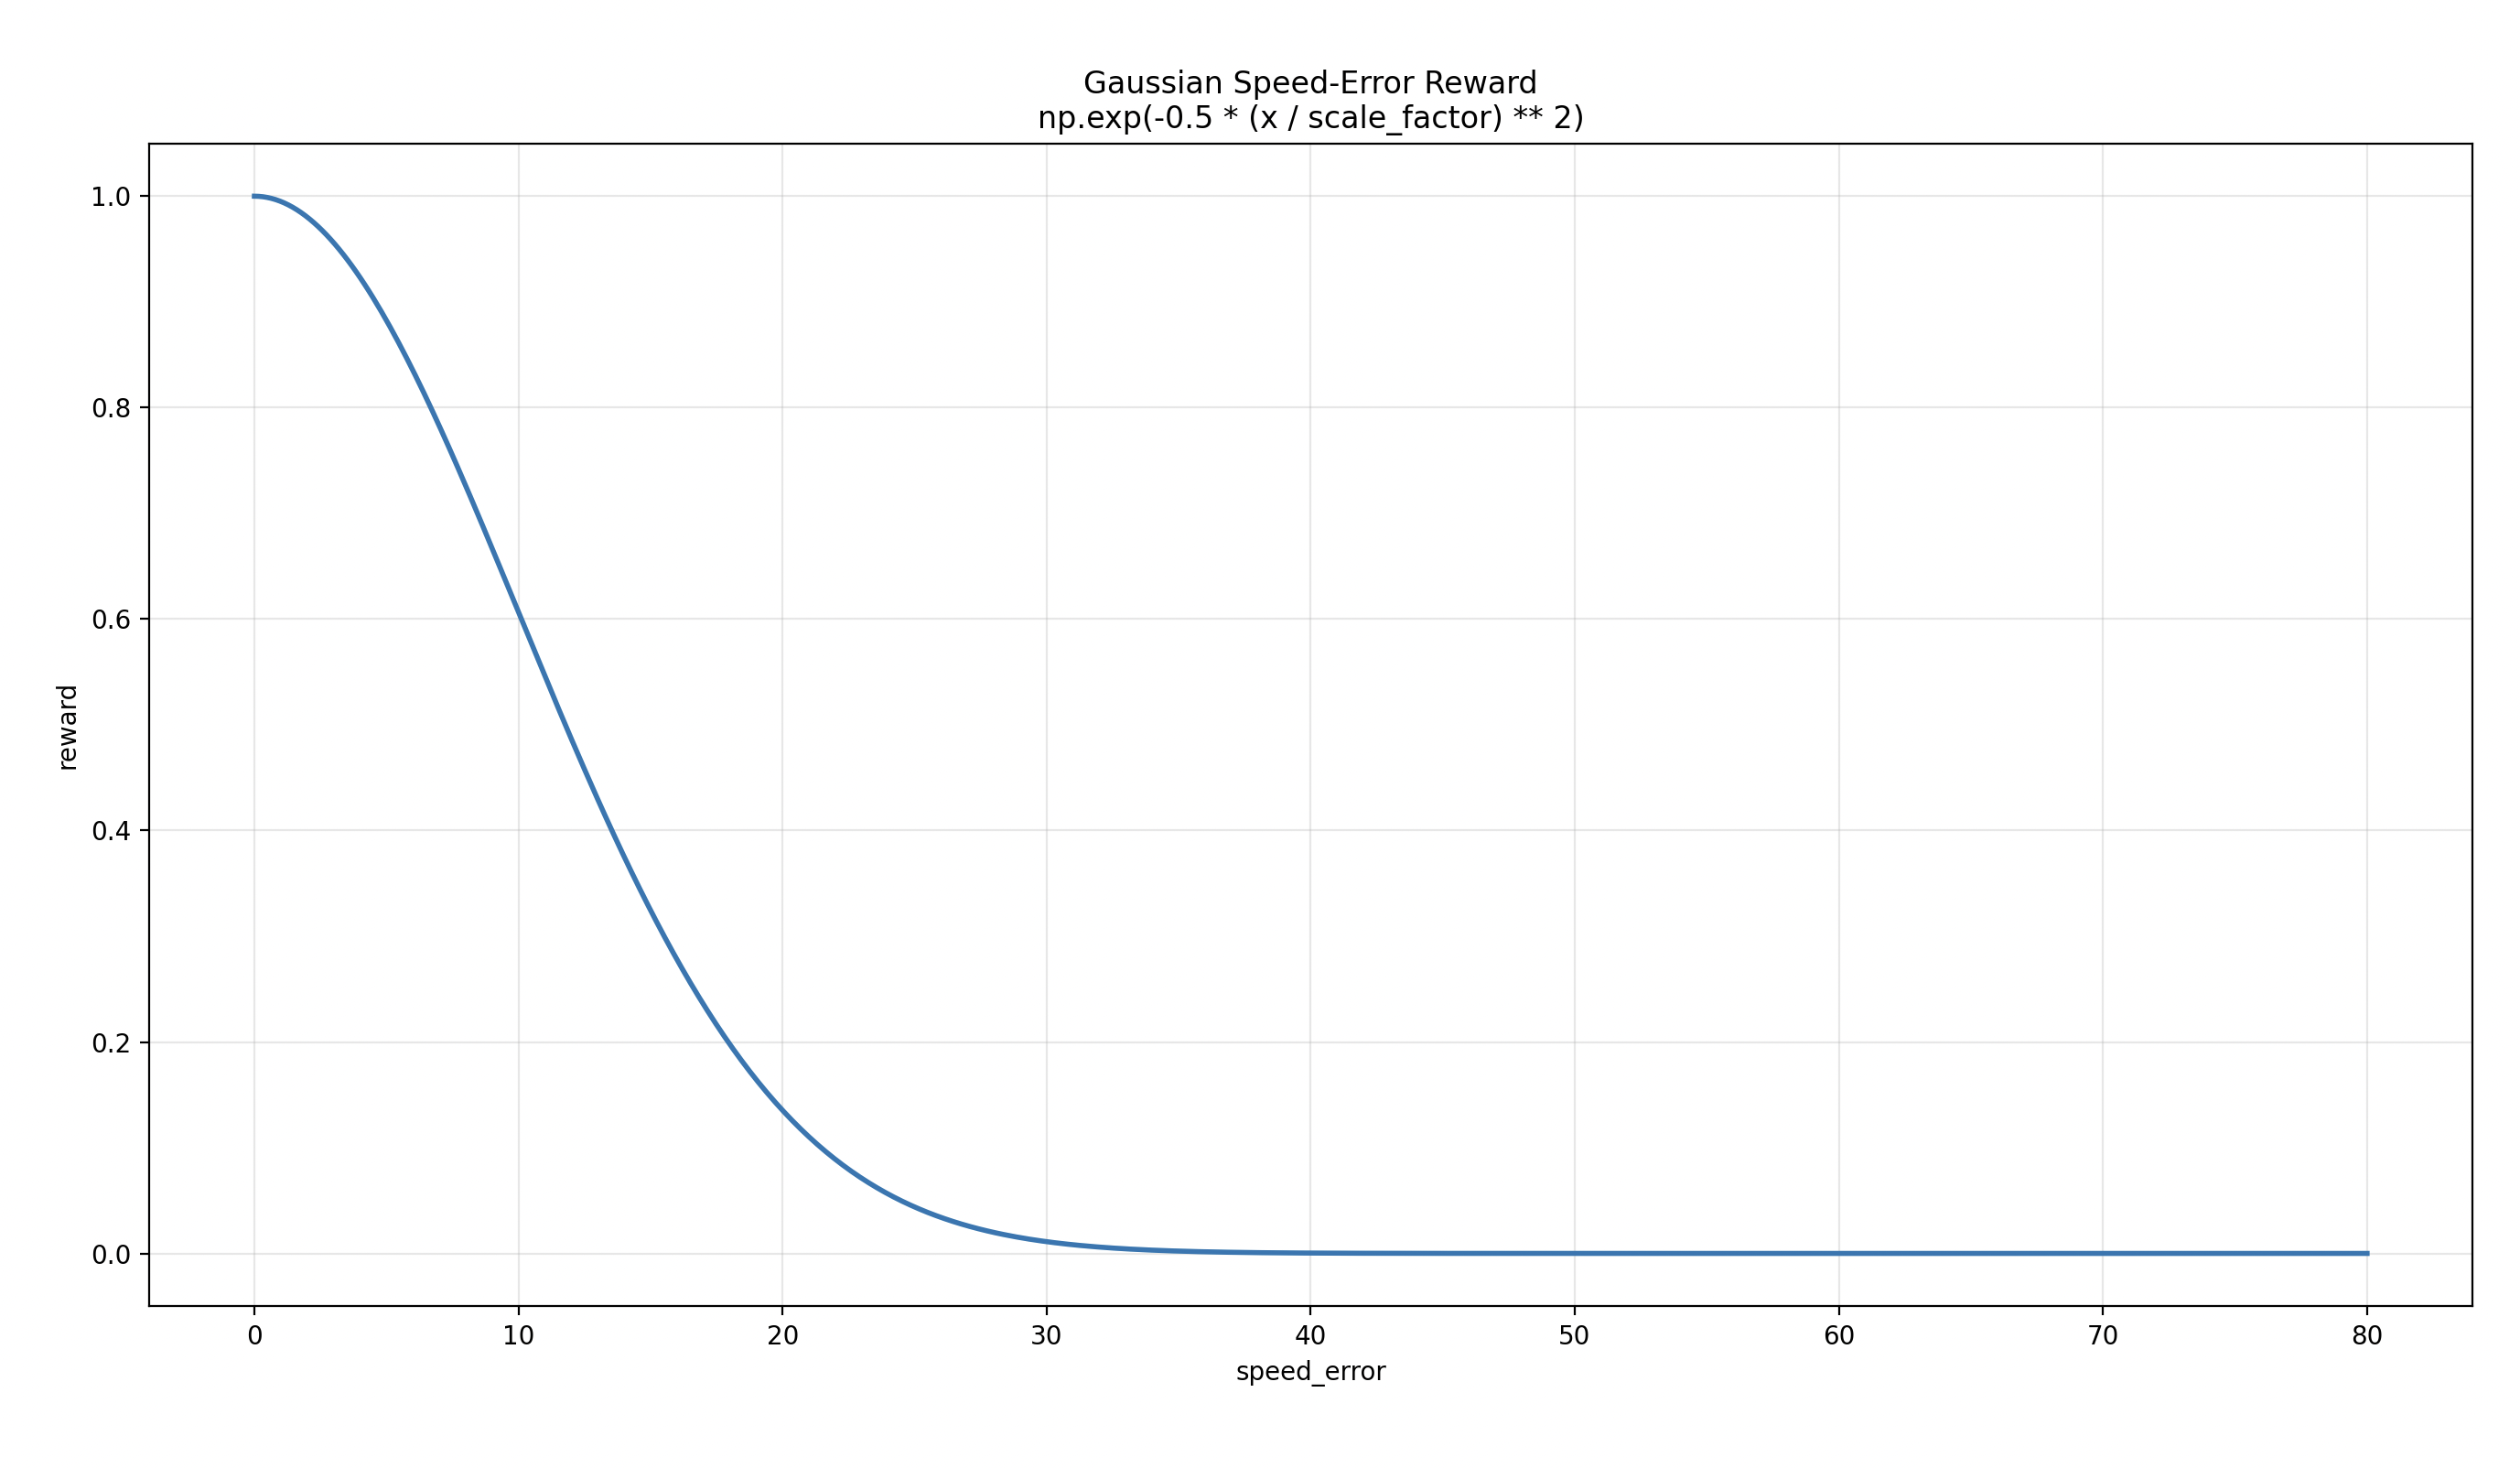
\includegraphics[width=0.75\textwidth]{imgs/gaussian_scaling.png}
  \caption[Gaussian speed-tracking reward term]{Gaussian speed-tracking reward scaling for $\sigma_v = 10$~km/h. The reward reaches its maximum at zero speed error and decays smoothly as the absolute tracking error increases.}
  \label{fig:reward_gaussian_scaling}
\end{figure}

Two design choices in \autoref{eq:reward} deserve emphasis:
\begin{itemize}
  \item First, the speed term is a dense, bounded bell in $[0,1]$ centred at zero error rather than a quadratic or absolute penalty: this keeps the tracking contribution from saturating the return at large transient errors while preserving a strong gradient close to the reference.
  \item Second, the emission term is clipped at $1$ with the $\min()$ operator inside $\tilde e_{\mathrm{NO}_{x},t}$, which caps the per-step penalty whenever the surrogate model produces an anomalously large tailpipe \ac{NOx} mass-flow prediction. This ensures stability against single outliers that might disrupt a smooth reward signal. The squared \ac{SOC} term penalises depletion and over-charging symmetrically around the episode-initial \ac{SOC} while penalising higher deviation stronger than minor in order to ensure that the agent is still able to use the electric motor to some extent. This term implements the charge-sustaining objective motivated in \autoref{subsec:method_reward}.
\end{itemize}

The per-phase weights are listed in \autoref{tab:reward_weights}. Phase~1 activates only the speed term and the mechanical shaping penalty, so that the agent first learns speed tracking in isolation, as motivated in \autoref{subsec:method_phase1}. Phase~2 additionally activates the emission and \ac{SOC} terms; their weights are first explored on a coarse $3\!\times\!3$ grid over $(W_{\text{emi}}, W_{\text{soc}^2})$ and subsequently refined by an Optuna-based search over the continuous ranges given in the last column of \autoref{tab:reward_weights}. The search procedure itself is described in \autoref{subsec:impl_phase2_pipeline}.

\begin{table}[H]
  \centering
  \small
  \begin{tabular}{|l|c|c|c|}
    \hline
    \textbf{Weight} & \textbf{Phase~1} & \textbf{Phase~2 grid} & \textbf{Phase~2 Optuna range} \\
    \hline
    $W_{\text{speed}}$ & $1.0$  & $1.0$                  & $1.0$ \\
    $W_{\text{emi}}$   & $0.0$  & $\{0.25,\,0.5,\,1.0\}$ & $[0.25,\,1.25]$ \\
    $W_{\text{soc}^2}$ & $0.0$  & $\{50,\,150,\,400\}$   & $[25,\,250]$ \\
    $W_{\text{brake}}$ & $0.25$ & $0.25$                 & $0.25$ \\
    $W_{\text{flick}}$ & $0.25$ & $0.25$                 & $0.25$ \\
    \hline
  \end{tabular}
  \caption[Reward weights per training phase]{Reward weights per training phase. Phase~1 keeps the emission and SOC terms inactive to isolate speed tracking. Phase~2 activates them and optimises their weights. Default values are stored in \texttt{config\_rewards.py}.}
  \label{tab:reward_weights}
\end{table}

With the Phase~1 weights of \autoref{tab:reward_weights}, the reward consists of the Gaussian speed-tracking term with $W_{\text{speed}} = 1.0$ and $\sigma_v = 10$~km/h, together with the two mechanical shaping penalties ($W_{\text{brake}} = 0.25$ and $W_{\text{flick}} = 0.25$), while the emission and \ac{SOC} penalties are disabled ($W_{\text{emi}} = W_{\text{soc}^2} = 0$). The maximum per-step reward is therefore $1.0$, achieved at zero speed error ($\Delta v_t = 0$), so the theoretical reward ceiling over a $1{,}800$\,s episode sampled at $2$\,Hz ($3{,}600$ simulation steps) is $3{,}600$. How closely the trained policies approach this ceiling is discussed in \autoref{sec:results_phase1}.

\paragraph{Safety mechanisms.}
Three additional mechanisms enforce that the surrogate networks remain inside their validated operating domain and that mechanically implausible actuation is suppressed.

\begin{itemize}
  \item \textbf{Hard \ac{SOC} clip.} The drivetrain output $\mathrm{SOC}_t$ is hard-clipped to $[0.0001, 0.9999]$ before being written back to the observation. This prevents the recurrent state of the drivetrain \ac{LSTM} from drifting into the unphysical boundary regions $\{0,\,1\}$, where the surrogate's prediction is not validated. These restrictions are not inherent artefacts of the \ac{LSTM}s; rather, they follow from how the surrogates were trained and were communicated orally by Frey et al. \cite{frey_data-based_2025} during preparation for this thesis.
  \item \textbf{Action safety filter.} When $\mathrm{SOC}_t$ is within $0.02$ of either boundary, the \ac{EM2} torque is overridden to zero if its sign would worsen the boundary violation: charging ($\tau_{EM2} < 0$) is blocked at $\mathrm{SOC}_t \ge 0.98$, and discharging ($\tau_{EM2} > 0$) is blocked at $\mathrm{SOC}_t \le 0.02$. This guarantees that the agent cannot drive the battery model beyond its validated window even before the hard clip takes effect. Although this measure is partly redundant with the hard \ac{SOC} clip, it provides an additional safety layer.
  \item \textbf{Engine switch cooldown.} The engine on/off state must remain unchanged for at least six consecutive simulation steps ($3\,\text{s}$ at $2\,\text{Hz}$). When the agent requests a transition before this window has elapsed, the requested state is overridden by the previous one and the engine-on default is set to the lower valid bounds $(n_{ICE},\,m_{fuel}) = (900\,\text{rpm},\,3\,\text{mg})$. Whenever the engine is off, both $n_{ICE}$ and $m_{fuel}$ are forced to zero regardless of the agent's commands. Following the conceptualisation of Alshiekh et al., this can be considered a post-posed shield: the shield is placed after the learning agent, monitors the selected action, and substitutes a safe action only if the agent's choice violates the safety specification \cite{alshiekh_safe_2017}. This ensures that the engine state is not toggled more frequently than physically feasible and avoids unrealistic engine wear.
\end{itemize}

\paragraph{Episode structure.}
All episodes are simulated at the surrogate sampling rate of $2\,\text{Hz}$ and span $N = 3{,}600$ steps, corresponding to $1{,}800\,\text{s}$ of vehicle operation. The target-speed schedule is configured differently for training and evaluation:

\begin{itemize}
  \item \textbf{Training.} The environment is constructed with \texttt{random\_target=True}. Each episode is split into six $600$-step segments ($300\,\text{s}$ each) and a new target speed is drawn uniformly from $[0,\,150]\,\text{km/h}$ at the start of every segment. Exposing the policy to many such randomised schedules spans a broad range of step transitions and steady-speed operating points.
  \item \textbf{Evaluation.} The environment is constructed with \texttt{eval\_mode=True} and uses the fixed deterministic schedule shown in \autoref{fig:six_phase_trajectory}. The six segments are each held for $600$ steps, supporting the deterministic and reproducible benchmarking discussed in \autoref{sec:method_evaluation}.
\end{itemize}

On every \texttt{reset()} call, the environment also re-initialises the recurrent state of both plant \ac{LSTM}s through the two-part initialisation scheme described in \autoref{sec:impl_lstms}. The initialisation network is supplied with physically meaningful initial conditions (zero emissions, ambient temperatures at $298\,\text{K}$, no \ac{ICE} torque, vehicle at rest, $\mathrm{SOC}_0 = 0.7$ unless overridden by the cycle file), which are mapped to hidden states compatible with the inference network. The observable-state attributes (last actions, last speed, last \ac{SOC}, last \ac{NOx} and last SCR1 temperature) are reset consistently with these initial conditions.

% ---------------------------------------------------------------------
\section{The Reinforcement-Learning Algorithms}
\label{sec:impl_algorithms}
The three reinforcement-learning algorithms selected in \autoref{subsec:method_algo_selection}, namely \ac{PPO}, \ac{TD3}, and \ac{SAC}, are implemented through the Stable-Baselines3 (SB3) library \cite{raffin_stable-baselines3_2021}. The actor and critic networks are multi-layer perceptrons (SB3's \texttt{MlpPolicy}); their hidden-layer widths and depths are not fixed manually but are treated as hyperparameters in the Phase~1 search. PPO uses a shared feature extractor for actor and critic, whereas SAC and TD3 use separate actor and twin-critic networks. Each agent observes the $12$-dimensional observation space, acts on the $4$-dimensional action space defined in \autoref{sec:impl_environment}, and is trained with the vectorised environment and normalisation wrappers described in \autoref{sec:impl_infrastructure}.

Apart from selecting the algorithm families and defining the heuristic hyperparameter-search spaces, no final agent configuration was chosen manually. Network widths, learning rates, batch sizes, update frequencies, exploration/noise parameters, and algorithm-specific options are therefore treated as outcomes of the Phase~1 hyperparameter optimisation described in \autoref{sec:impl_hpo}. The algorithmic mechanics are introduced in \autoref{chap:theory}, the selection rationale is given in \autoref{subsec:method_algo_selection}, and the resulting per-algorithm configurations are reported in Appendix~\ref{app:phase1_hyperparams} (\autoref{tab:phase1_best_hyperparameters}).

% ---------------------------------------------------------------------
\section{Optuna Hyperparameter Optimisation}
\label{sec:impl_hpo}

Each Phase-1 algorithm is tuned through an independent Optuna study that minimises the deterministic speed-tracking \ac{RMSE} on the evaluation cycle (\autoref{sec:method_evaluation}). Optimising the measured task metric rather than the shaped reward avoids selecting configurations that exploit the reward design, so called reward hacking (\autoref{subsec:method_reward}) \cite{pan_effects_2022}. The Phase~2 reward search, however, minimises the composite score $J$ (\autoref{eq:phase2_objective}). The remaining setup is kept consistent.

\paragraph{Sampler, pruner and storage.}
The studies use a \ac{TPE} sampler (\texttt{TPESampler}) with ten random startup trials before the Bayesian phase, and a \texttt{MedianPruner} with a warm-up of $2{,}000{,}000$ timesteps, a reporting interval of $500{,}000$ timesteps and five startup trials. After the warm-up, an evaluation callback runs five deterministic episodes at every reporting interval, computes the pooled \ac{RMSE} and reports it to the pruner. Trials whose intermediate \ac{RMSE} is worse than the median of completed trials at the same step are pruned. The study state is persisted to an append-only \texttt{JournalStorage} log file, which is crash-safe and can be shared across SLURM-array workers (\autoref{sec:impl_infrastructure}) without a separate database service.

\paragraph{Budget and search spaces.}
Each trial trains a candidate agent for a total of $4{,}000{,}000$ timesteps in the vectorised training environment described in \autoref{sec:impl_infrastructure}. A budget of $20$ trials per study is allocated for each of the three algorithms, although the actual number of completed trials differs, as explained in \autoref{sec:limitations_of_the_study}. The algorithm-specific search spaces are listed in Appendix~\ref{app:phase1_hyperparams}, \autoref{tab:hpo_search_spaces}.

\paragraph{Outputs.}
Each study persists two artefacts: \texttt{best\_params.json} as the resolved best-trial parameters, and \texttt{all\_trials.csv} as the per-job record. The selected best hyperparameters per algorithm are represented in Appendix~\ref{app:phase1_hyperparams}, \autoref{tab:phase1_best_hyperparameters}.

% ---------------------------------------------------------------------
\section{Training Infrastructure}
\label{sec:impl_infrastructure}

\paragraph{Cluster execution.}
All training runs are dispatched as SLURM array jobs. Each array worker instantiates the same Optuna study via the shared \texttt{JournalStorage} (\autoref{sec:impl_hpo}), so multiple Phase-1 trials proceed in parallel without coordination beyond the shared journal log.

\paragraph{Environment vectorisation.}
At runtime, the custom \texttt{EmissionControlEnv} is wrapped in an SB3 \texttt{SubprocVecEnv}, which executes $n_{\text{envs}}$ instances of the environment in parallel worker processes. $n_{\text{envs}}$ is set to $20$ during hyperparameter search and multi-seed validation. The seed of each child environment is derived from the run identifier to avoid correlated initial conditions across workers while preserving full reproducibility.

\paragraph{Observation and reward normalisation.}
The environment is wrapped in \texttt{VecNormalize}, which maintains running statistics of observations and rewards. Observations are always normalised (based on the min-max values in \autoref{tab:obs_vector}); reward normalisation is enabled only for PPO, since the off-policy algorithms would be destabilised by rescaling of past experiences when sampling from their replay buffers. The running statistics are persisted alongside each model checkpoint as \texttt{vec\_normalize.pkl} so that any downstream evaluation or fine-tuning can reload them and reproduce the same observation distribution.

\paragraph{Checkpointing and provenance.}
Training is monitored by SB3's \texttt{CheckpointCallback} and a custom callback that produces \texttt{vec\_normalize.pkl} with a frequency of $100{,}000$ timesteps. At the end of each run, the final model, the final normaliser, the evaluation metrics\linebreak(\texttt{evaluation\_metrics.json}) and a record of the training config (\texttt{train\_config.json}) are written to the run directory. The record of the training config stores the algorithm, the random seed, the active reward weights, the training duration and the override-source paths, which allows downstream analyses.

% ---------------------------------------------------------------------
\section{Per-Phase Implementation Pipelines}
\label{sec:impl_pipelines}

\subsection{Phase~1 Pipeline}
\label{subsec:impl_phase1_pipeline}
Phase~1 fixes the reward to the speed-only objective (\autoref{tab:reward_weights}) and is realised as a three-stage pipeline. The stages are decoupled into separate launchers so that they can be dispatched independently as SLURM array jobs:

\begin{enumerate}
  \item \textbf{Hyperparameter optimisation.} One Optuna study is launched per algorithm over the search spaces in \autoref{tab:hpo_search_spaces}, minimising deterministic speed-tracking \ac{RMSE}. Each trial trains a fresh agent for $4{,}000{,}000$ timesteps on $20$ parallel environments, evaluates it on the deterministic six-phase cycle every $500{,}000$ timesteps, and reports the result to a median pruner. The selected hyperparameters and trial history are saved as \texttt{best\_params.json} and \texttt{all\_trials.csv}.
  \item \textbf{Multi-seed validation.} The winning \texttt{best\_params.json} is trained $10$ times with seeds $\{0,\,\dots,\,9\}$, one seed per array task. Each seed run executes $4{,}000{,}000$ timesteps, checkpoints the model and \texttt{vec\_normalize.pkl} every $100{,}000$ steps, and writes the final model, normaliser, \linebreak\texttt{train\_config.json}, and deterministic \texttt{evaluation\_metrics.json}.
  \item \textbf{Best-seed selection.} The per-seed evaluation files are ranked by $\mathrm{RMSE}_v$ so the lowest speed-tracking \ac{RMSE} is selected and ties are broken by lower cumulative \ac{NOx}. The corresponding model checkpoint and \texttt{vec\_normalize.pkl} form the bridge to Phase~2.
\end{enumerate}

\begin{figure}[htbp]
  \centering
  \includestandalone[width=0.7\textwidth]{tikz/phase1}
  \caption[Technical pipeline of Phase~1]{Technical pipeline of Phase~1.}
  \label{fig:phase1}
\end{figure}

\subsection{Phase~2 Pipeline}
\label{subsec:impl_phase2_pipeline}
Phase~2 reuses the Phase~1 best-seed checkpoint as a fine-tuning warm-start (\autoref{subsec:method_phase2}) and activates the additional \ac{NOx} and squared-\ac{SOC} reward terms from \autoref{tab:reward_weights}. It is implemented as a three-stage pipeline whose runs can again be dispatched independently as SLURM array jobs:

\begin{enumerate}
  \item \textbf{Warm-start fine-tune.} Each Phase~2 run loads the Phase~1 \texttt{final.zip} checkpoint and its \texttt{vec\_normalize.pkl} normaliser into a freshly constructed Phase~2 environment. The Phase~1 hyperparameters are reapplied, while \texttt{learning\_starts} is deliberately omitted from the reload arguments to avoid a second random-action warm-up.
  \item \textbf{Reward-weight study.} The emission and \ac{SOC} weights are first explored with a $3\!\times\!3$ grid, $(W_{\text{emi}},\,W_{\text{soc}^2}) \in \{0.25,\,0.5,\,1.0\}\times\{50,\,150,\,400\}$, with one grid cell per SLURM array task. Each cell fine-tunes the Phase~1 checkpoint for $4{,}000{,}000$ timesteps, evaluates on the deterministic six-phase cycle, and saves per-cell artefacts. Because this grid samples only nine fixed combinations, it is followed by a per-algorithm Optuna search over $W_{\text{emi}} \in [0.25,\,1.25]$ and $W_{\text{soc}^2} \in [25,\,250]$, using the same \ac{TPE} sampler, median pruner and \texttt{JournalStorage} setup as Phase~1. Each Optuna trial samples one weight pair, fine-tunes for $4{,}000{,}000$ timesteps, evaluates every $500{,}000$ timesteps, and minimises the constrained score in \autoref{eq:phase2_objective}.
  \item \textbf{Multi-seed validation.} The selected weight pair from \texttt{best\_params\_phase2.json} is validated across seeds $\{0,\,\dots,\,9\}$, one seed per array task. Each seed continues from the same Phase~1 checkpoint, trains for $4{,}000{,}000$ timesteps over $20$ parallel environments, and writes the final model, \texttt{vec\_normalize.pkl}, \texttt{train\_config.json}, and deterministic \linebreak\texttt{evaluation\_metrics.json}.
\end{enumerate}

\paragraph{Composite score for multi-objective optimisation.}
The Optuna reward-weight score used in Stage~2 is

\begin{equation}
  J = M_{\mathrm{NO}_{x},\mathrm{tp}}^{\mathrm{eval}}
  + \lambda_{\text{RMSE}}\,\max\!\bigl(0,\,\mathrm{RMSE}_v - r_{\text{RMSE}}\bigr)^{2}
  + \lambda_{\text{SOC}}\,\max\!\bigl(0,\,\max_t|\Delta\mathrm{SOC}_t| - r_{\text{SOC}}\bigr)^{2},
  \label{eq:phase2_objective}
\end{equation}

where $M_{\mathrm{NO}_{x},\mathrm{tp}}^{\mathrm{eval}}$ is the cumulative tailpipe \ac{NOx} mass in grams over the deterministic evaluation cycle. It is obtained from the instantaneous surrogate output $\dot m_{\mathrm{NO}_{x},\mathrm{tp},t}$ as

\begin{equation}
  M_{\mathrm{NO}_{x},\mathrm{tp}}^{\mathrm{eval}}
  = \sum_{t=0}^{T-1} \dot m_{\mathrm{NO}_{x},\mathrm{tp},t}\,\Delta t,
  \label{eq:cumulative_nox_eval}
\end{equation}

and corresponds to the evaluation metric stored as \texttt{total\_nox\_g}, not the instantaneous g/s \ac{LSTM} output. The term $\mathrm{RMSE}_v$ is the evaluation speed-tracking \ac{RMSE} in km/h, and $\max_t|\Delta\mathrm{SOC}_t|$ is the peak \ac{SOC} drift over the cycle. The fixed constants are $\lambda_{\text{RMSE}} = 20$, $\lambda_{\text{SOC}} = 1000$, $r_{\text{RMSE}} = 5\,\text{km/h}$, and $r_{\text{SOC}} = 0.05$; lower scores are better.

The composite score combines three design elements:
\begin{itemize}
  \item \textbf{Scalarisation.} The simultaneously considered objectives are transformed into a single scalar objective that Optuna can minimise \cite{helfrich_using_2024}.
  \item \textbf{$\epsilon$-constraint formulation.} Cumulative tailpipe \ac{NOx} remains the primary objective, while speed-tracking error and \ac{SOC} drift are treated as constraints with tolerances $r_{\text{RMSE}}$ and $r_{\text{SOC}}$ \cite{haimes_bicriterion_1971}.
  \item \textbf{Quadratic penalties.} Constraint violations outside these tolerances are penalised quadratically, so feasible deviations are ignored while larger violations become increasingly costly.
\end{itemize}

Together, these elements make cumulative tailpipe \ac{NOx} the primary objective and treat speed tracking and charge sustainment as soft constraints. Within the tolerances, the penalties vanish; outside them, they grow quadratically. The tolerances are set relative to Phase~1: its best seeds achieve $3.1$--$3.5\,\text{km/h}$ \ac{RMSE} (\autoref{sec:results_phase1}), so $r_{\text{RMSE}} = 5\,\text{km/h}$ leaves a moderate tracking margin. In contrast, $r_{\text{SOC}} = 0.05$ is far below the $\sim\!0.30$ saturation drift observed in Phase~1 and therefore discourages the battery-exploitation behaviour that motivates Phase~2 (\autoref{subsec:method_phase2}).

The two coefficients $\lambda_{\text{RMSE}}$ and $\lambda_{\text{SOC}}$ exist only to place the three terms on a common scale. The cumulative \ac{NOx} values being minimised are on the order of a few grams, so clear constraint violations must add comparable or larger costs; otherwise, the \ac{NOx} term would dominate and Optuna could accept poor tracking or excessive \ac{SOC} drift. The difficulty is that the two penalised quantities are numerically very different: a speed-error excess is measured in km/h and squares to values of order $1$ to $10$, whereas a \ac{SOC}-drift excess is a small fraction and squares to values of order $10^{-3}$ to $10^{-2}$. A shared multiplier would therefore render the \ac{SOC} term negligible. The choice $\lambda_{\text{RMSE}} = 20$ and $\lambda_{\text{SOC}} = 1000$ offsets this scale gap: at a clear violation each term becomes large enough to steer the search away from infeasible weights. For example, a $2\,\text{km/h}$ tracking excess adds $20 \cdot 2^2 = 80$ units, while a $0.10$ \ac{SOC}-drift excess adds $1000 \cdot 0.1^2 = 10$ units. The larger \ac{SOC} coefficient merely compensates for its far smaller squared scale; it does not make \ac{SOC} the more important constraint. The asymmetry in the resulting magnitudes ($80$ versus $10$) is intentional: \ac{RMSE} acts as a hard wall against catastrophic forgetting, while the softer \ac{SOC} term allows more flexibility.

\begin{figure}[htbp]
  \centering
  \includestandalone[width=0.7\textwidth]{tikz/phase2}
  \caption[Technical pipeline of Phase~2]{Technical pipeline of Phase~2.}
  \label{fig:phase2}
\end{figure}
